\documentclass[12pt]{article}
%\documentclass[12pt]{abntex2}


\usepackage{amssymb,amsmath,amsfonts,eurosym,geometry,ulem,graphicx,caption,color,setspace,sectsty,comment,footmisc,caption,natbib,pdflscape,subfigure,array,hyperref}
%\usepackage[brazilian,hyperpageref]{backref}	 % Paginas com as citações na bibl
\usepackage{lscape}
\usepackage{wallpaper}
\usepackage{pdfpages}			% Inclui anexos em pdf
\usepackage{pdflscape}
\usepackage{longtable}
\usepackage{booktabs}
\usepackage{float}
\usepackage{hyperref}
\usepackage{backref}

\graphicspath{{figures/}{../Propose/R/RAIS/figures/}{../Propose/R/figures/}{../Propose/replication/HPV Brazil code/figures/}{../replication/HPV code/baseline/}}
\newcommand{\citeonline}[1]{\citet{#1}}

% ---
% Configurações do pacote backref
% Usado sem a opção hyperpageref de backref
\renewcommand{\backrefpagesname}{Citado na(s) página(s):~}
% Texto padrão antes do número das páginas
\renewcommand{\backref}{}
% Define os textos da citação
\renewcommand*{\backrefalt}[4]{
	\ifcase #1 %
	Nenhuma citação no texto.%
	\or
	Citado na página #2.%
	\else
	Citado #1 vezes nas páginas #2.%
	\fi}%
% ---

\hypersetup{
	%pagebackref=true,
	pdftitle={Business Cycle and Inequality in Emerging Economies}, 
	pdfauthor={Matheus Porto Pimentel},
	pdfsubject={Business cycles, labor income inequality, and RAIS microdata},
	pdfcreator={LaTeX with abnTeX2},
	pdfkeywords={abnt}{latex}{abntex}{abntex2}{trabalho acadêmico}, 
	colorlinks=true,       		% false: boxed links; true: colored links
	linkcolor=blue,          	% color of internal links
	citecolor=blue,        		% color of links to bibliography
	filecolor=magenta,      		% color of file links
	urlcolor=blue,
	bookmarksdepth=4
}
\makeatother
% --- 

\normalem

\onehalfspacing
\newtheorem{theorem}{Theorem}
\newtheorem{corollary}[theorem]{Corollary}
\newtheorem{proposition}{Proposition}
\newenvironment{proof}[1][Proof]{\noindent\textbf{#1.} }{\ \rule{0.5em}{0.5em}}

\newtheorem{hyp}{Hypothesis}
\newtheorem{subhyp}{Hypothesis}[hyp]
\renewcommand{\thesubhyp}{\thehyp\alph{subhyp}}

\newcommand{\red}[1]{{\color{red} #1}}
\newcommand{\blue}[1]{{\color{blue} #1}}

\newcolumntype{L}[1]{>{\raggedright\let\newline\\arraybackslash\hspace{0pt}}m{#1}}
\newcolumntype{C}[1]{>{\centering\let\newline\\arraybackslash\hspace{0pt}}m{#1}}
\newcolumntype{R}[1]{>{\raggedleft\let\newline\\arraybackslash\hspace{0pt}}m{#1}}

\geometry{left=1.0in,right=1.0in,top=1.0in,bottom=1.0in}

\begin{document}
	
	\begin{titlepage}
		\title{Business Cycle and Inequality in Emerging Economies\thanks{This
				study was financed in part by the Coordenação de Aperfeiçoamento de Pessoal de Nível Superior - Brasil
				(CAPES) - Finance Code 001.}}
		\author{Matheus Porto Pimentel  \thanks{EPGE Brazilian School of Economics and Finance.
				\textbf{E-mail address:} matheusportopimentel@gmail.com} and Pedro Poliseli \thanks{EPGE Brazilian School of Economics and Finance.}}
		\date{\today}
		\maketitle
		\begin{abstract}
			\noindent 
			This paper studies how business-cycle fluctuations shape labor-income inequality in Brazil. We adapt the framework of \citeonline{heathcote2020rise} to an emerging economy with high baseline inequality, recurrent aggregate volatility, and a large formalization episode during the 2000s. Relative to Heathcote, Perri, and Violante, our contribution is empirical and quantitative in three dimensions. First, we document the evolution of the Brazilian formal earnings distribution using RAIS administrative records for prime-age men from 1994 to 2022, measuring earnings percentiles in multiples of the minimum wage. Second, we estimate labor-market transition matrices directly from PNAD Continua microdata for Brazil, matching adjacent quarters from 2012 to 2024 and distinguishing employment, unemployment, and non-participation. Third, we construct Brazil-specific model objects for the transition block: aggregate states are defined using GDP at market prices from IBGE/SIDRA, crisis years are set to 2015, 2016, and 2020, and workers are classified by education into low-, mid-, and high-skill groups. The resulting calibration differs from the U.S. application in both the data source and the economic mechanism emphasized. While the U.S. evidence highlights rising inequality associated with declining participation among low-earning men, the Brazilian evidence shows strong compression of formal earnings in multiples of the minimum wage and marked heterogeneity in transition probabilities by education and cycle state. The paper provides a first step toward a structural evaluation of how recessions, recoveries, and worker heterogeneity interact in shaping inequality in Brazil.
			\\
			\vspace{0in}\\
			\noindent\textbf{Keywords:} business cycles, earnings inequality, labor-market transitions, RAIS,\\ PNAD Continua, Brazil\\
			\vspace{0in}\\
			\noindent\textbf{JEL Codes:} E24, E32, J21, J24, J31, O54\\
			
			\bigskip
		\end{abstract}
		\setcounter{page}{0}
		\thispagestyle{empty}
	\end{titlepage}
	\pagebreak \newpage
	
	\doublespacing
	
	
	\section{Introduction} \label{sec:introduction}
	
	%# Introduction
	
	Income inequality remains one of the defining characteristics of the Brazilian economy. Despite substantial economic and institutional transformations in recent decades, large disparities in earnings persist between workers, sectors, and regions. 
	
	
	At the same time, the Brazilian economy has experienced recurrent episodes of expansion and recession, generating significant fluctuations in employment, wages, and labor market participation. These observations raise a fundamental question: how do business cycle fluctuations affect the distribution of labor income and, ultimately, the evolution of inequality?
	
	This paper studies the relationship between business cycle dynamics, labor market outcomes, and income inequality in Brazil. We argue that aggregate economic fluctuations affect workers heterogeneously, generating distributional consequences that extend beyond their aggregate effects on employment and output. During downturns, labor market adjustments may disproportionately affect specific groups of workers through changes in unemployment, labor force participation, job reallocation, and wage dynamics. Conversely, economic expansions may generate unequal gains across workers depending on their position in the earnings distribution and their attachment to the labor market. Understanding these mechanisms is essential for evaluating the distributional effects of macroeconomic shocks and the role of stabilization policies in economies characterized by high levels of inequality.
	
	To address this question, we develop a model in which business cycle shocks propagate through the labor market and affect the distribution of labor income. The framework in this paper builds on
	\citeonline{heathcote2020rise}. The framework captures the interaction between aggregate fluctuations and heterogeneous labor market outcomes, allowing us to characterize the channels through which cyclical movements influence inequality. The model highlights how changes in labor demand translate into differential employment and wage responses across workers, generating time-varying income dispersion over the business cycle.
	
	The theoretical analysis is complemented by an empirical investigation using Brazilian labor market data. The empirical exercise exploits detailed worker-level information to document the cyclical behavior of employment, earnings, and measures of inequality. We examine how labor market transitions and wage adjustments contribute to changes in income dispersion during periods of economic expansion and contraction. This approach allows us to evaluate the extent to which the mechanisms emphasized by the model are supported by the data.
	
	Our preliminary findings indicate that business cycle fluctuations have important distributional consequences. Economic downturns are associated with disproportionate employment losses among lower-income workers, while wage adjustments are concentrated among workers located at different points of the earnings distribution. As a result, recessions tend to increase measures of inequality, whereas expansions generate more heterogeneous effects depending on the source of economic growth and the composition of employment gains. These results suggest that aggregate fluctuations influence not only the level of economic activity but also the distribution of income across households.
	
	This paper contributes to the literature in three dimensions. First, it contributes to the growing literature that studies the distributional consequences of business cycle fluctuations by emphasizing the labor market as the primary transmission mechanism between aggregate shocks and inequality. Second, it contributes to the literature on inequality in developing economies by providing new evidence for Brazil, a country characterized by persistent income disparities and substantial labor market heterogeneity. Third, it combines a theoretical framework with micro-level evidence, allowing for a unified analysis of the mechanisms linking macroeconomic fluctuations to the evolution of inequality.
	
	The Brazilian case provides a particularly relevant environment in which to study these issues. The combination of high baseline inequality, large labor market informality, and recurrent macroeconomic volatility offers a unique opportunity to examine how aggregate shocks affect different groups of workers. Consequently, understanding the relationship between business cycles and inequality in Brazil may also provide insights applicable to other emerging economies facing similar structural characteristics.
	
	The remainder of the paper is organized as follows. Section 1.1 discusses the related literature. Section 2 describes the data and the empirical facts. Section 3 presents the model. Section 4 describes the calibration for Brazil. Section 5 will compare the empirical findings with the model implications. Section 6 concludes.
	
	
	%The phenomenon of inequality has spread throughout the world. Advanced economics has faced numerous increases in inequality in recent decades. 
	
	%O fenomeno da desigualdade vem se espalhando pelo mundo. Economias avançadas tem se deparado com crescente aumento da desigualdade nas décadas recentes. O mesmo vêm acontecendo em economias emergentes, tais como o Brasil e países da América Latina (talvez BRICS?) Falar sobre quem já documentou isso na literatura. O objetivo deste trabalho é compreender/documentar como a desigualdade vem impactando o desenvolvimento assimétrico em países em desenvolvimento. No Brasil vários trabalhos tem abordado de maneira reduzida/microeconometricamente. Pretendo avaliar esse fenômeno através de um modelo de equilibrio geral e estrutural e como o ciclo de negócios impacta o rendimento dos trabalhadores além das decisões de participação ou não na força de trabalho. 
	
	%\citeonline{heathcote2020rise}  encotram que a maior fonte de aumento da desigualdade de renda nos Estados Unidos se deve a redução das horas trabalhadas por homens na metade inferior da distribuição de renda. A redução de horas trabalhadas é causada em grande parte nas recessões onde os  salários caem e não se recuperam totalmente em expansões. Todavia, essas conclusões foram realizadas antes da pandemia de covid-19 e para os Estados Unidos. No Brasil tivemos a recessão de 2015-2016 com potencial de impactar as decisões de participação ou não na força de trabalho, além do fato de que saídas temporárias da força de trabalho pode deixar cicatrizes permanentes nos rendicmentos desses trabalhadores.
	
	%Esses homens de baixa qualificação em recessões sofrem um golpe duplo, além de perder os rendimentos (desemprego) ainda depreciam suas habilidades o que deixa cicatrizes permanentes em recessões. Além disso, os trabalhadores nas recessões desistem de procurar emprego, o que causa a saídae
	%permanente do mercado de trabalho, redução da participação.
	
	%Tendência secular, em particular, dos efeitos da mudança tecnológica que em geral favoreceu trabalhadores com habilidades relativamente altas (pode ter papel significativo agora com o advento da IA). Flutuações ciclícas têm efeitos persistentes sobre a desigualdade de rendimentos como pontuam \citeonline{heathcote2020rise}. Argumentaremos que parte do aumento observado na desigualdade ao longo do último meio século pode ser atribuído as recessões no Brasil vivenciadas nos últimos anos. O Brasil é um país que vivenciou expansões, mas sobretudo recessões nas últimas décadas. Década de 1980, e mais recentemente 2015/2016 e a pandemia de covid-19. 
	
	%A desigualdade de renda hoje no Brasil poderia ser menor se o Brasil, tivesse de alguma forma, evitado recessões durante o período estudado. 
	
	%Desigualdade de renda pune mais os trabalhadores não qualificados, low skill. 
	
	%O progresso tecnológico é um fator fundamental para o crescimento econômico, ao mesmo tempo em que favorece trabalhadores mais qualificados. O que é um fator fundamental para o aumento da desigualdade, no topo.
	
	%Índices como o índice de Gini Global não são capazes de capturar a totalidade da complexidade de renda. É possível que olhando o índice a desigualdade brasileira nas últimas duas décadas tenha consistentemente caído, mas quando olhamos para o percentil 50/90 o aumento é significativo. 
	
	%Isso tudo ao mesmo tempo em que as flutuações no desemprego são um aspecto fundamental do ciclo econômico.
	
	
	
	%The rest of the paper is organized as follows. Section 2 describe the key facts about the distribution of earnings and hours of worked that we wain to explain. Section 3 outlines the model. Section 4 describes the model parametrization. Section 5 presents the results of the model simulations and counterfactuals. Section 6 concludes.
	
	\subsection{Related Literature}
	
	%# Related Literature
	
	This paper is closely related to a growing literature that studies the interaction between labor market dynamics, business cycle fluctuations, and income inequality. The main inspiration for our analysis is \citeonline{heathcote2020rise}, who document the rise of earnings inequality in the United States over the last five decades and emphasize the importance of labor market participation and hours worked in explaining this phenomenon. Their central finding is that a substantial share of the increase in income inequality is attributable to declining labor supply among men in the lower half of the earnings distribution. Importantly, recessions play a key role in this process. Adverse labor market conditions reduce employment and hours worked among low-skilled workers, while subsequent expansions fail to fully reverse these losses. As a result, cyclical downturns generate persistent distributional effects that accumulate over time.
	
	Our paper builds directly on this insight but shifts the focus to Brazil, a country characterized by substantially different labor market institutions, higher levels of informality, and a history of recurrent macroeconomic instability. While the mechanisms highlighted by \citeonline{heathcote2020rise} have been extensively documented for the United States, much less is known about the extent to which business cycle fluctuations contribute to long-run inequality dynamics in emerging economies. This question is particularly relevant in Brazil, where severe recessions such as those of 2015–2016 and the COVID-19 pandemic generated large increases in unemployment and significant disruptions in labor market participation.
	
	More broadly, this paper contributes to a literature that examines the causes and consequences of rising inequality. \citeonline{storesletten2020should} emphasize the importance of understanding inequality dynamics from both efficiency and welfare perspectives, highlighting the role of labor market risks and heterogeneous exposure to macroeconomic shocks. Similarly, \citeonline{heathcote2023more} provide evidence that changes in labor market outcomes remain a central driver of inequality trends, even in environments characterized by substantial policy interventions and structural economic change. Together, these studies reinforce the view that inequality cannot be understood solely through changes in wages or skill premia, but must also account for employment dynamics, participation decisions, and exposure to cyclical fluctuations.
	
	Another important strand of the literature focuses on the secular forces underlying inequality growth. A large body of research emphasizes skill-biased technological change as a major determinant of earnings dispersion. Technological progress increases productivity and promotes long-run economic growth, but often disproportionately benefits workers with higher levels of education and skills. These mechanisms have contributed to rising wage inequality in many countries and may become even more relevant with the diffusion of artificial intelligence and other advanced technologies. While technological change is typically viewed as a long-run force shaping inequality, our analysis argues that cyclical fluctuations interact with these secular trends. Recessions tend to disproportionately affect low-skilled workers, amplifying pre-existing inequalities generated by structural changes in labor demand.
	
	The paper also relates to the literature on labor market scarring. Workers who experience unemployment during recessions frequently suffer persistent earnings losses that extend well beyond the initial downturn. These effects are particularly pronounced among low-skilled workers, who face a double burden during economic contractions. In addition to the immediate loss of labor income associated with unemployment, prolonged detachment from employment may lead to human capital depreciation and weaker future labor market prospects. Recessions may therefore generate permanent reductions in earnings capacity, contributing to persistent increases in inequality. Moreover, adverse labor market conditions often discourage job search activity, leading some individuals to exit the labor force altogether. These participation responses further magnify the long-run distributional consequences of business cycle fluctuations.
	
	For Brazil, the literature remains comparatively limited. Two notable contributions are \citeonline{alvarez2018firms} and \citeonline{engbom2022earnings}, both of which study important dimensions of earnings inequality using matched employer-employee data. Their analyses provide valuable evidence on wage dynamics and the role of firms in shaping earnings dispersion. However, these studies do not explicitly investigate the interaction between business cycles, labor market participation, and inequality. Furthermore, both analyses are largely based on data preceding the COVID-19 pandemic and therefore capture only part of the economic disruptions associated with the deep recession of 2015–2016 and the subsequent pandemic shock.
	
	Our contribution differs from this literature in several dimensions. First, we explicitly connect business cycle fluctuations to the evolution of inequality through labor market mechanisms. Second, we analyze the Brazilian experience over a period that encompasses both the 2015–2016 recession and the COVID-19 crisis, two of the most severe economic contractions in recent Brazilian history. Third, we argue that conventional inequality measures, such as the Gini coefficient, may not fully capture the complexity of distributional changes over time. While some aggregate measures suggest declining inequality in Brazil during portions of the last two decades, alternative indicators based on earnings dispersion across percentiles reveal substantially different patterns. In particular, measures such as the 90/50 ratio indicate that important dimensions of inequality may have increased despite improvements in broader aggregate indicators.
	
	The central hypothesis of this paper is that business cycle fluctuations constitute an important and underappreciated source of long-run inequality. Recessions disproportionately affect low-skilled workers through unemployment, labor force withdrawal, and persistent earnings losses, while expansions only partially offset these effects. Consequently, part of the observed increase in inequality may reflect the cumulative impact of successive economic downturns. In this sense, the Brazilian experience provides a unique laboratory for understanding how repeated episodes of macroeconomic instability shape the distribution of income over time. Our results suggest that income inequality in Brazil could be substantially lower today had the economy experienced fewer or less severe recessions during the period under analysis.
	
	
	%Para o caso brasileiro temos \citeonline{alvarez2018firms} and \citeonline{engbom2022earnings}. Esses trabalhos olham substancialmente para dimensões de salário minímo sem observar questões estruturais e ciclos de negócios. Ambas as análises são anteriores a pandemia de covid-19 e capturaram apenas os efeitos parciais da crise vivida no Brasil entre 2015/2016.
	
	%No caso geral, outros importantes trabalhos sobre aumento de desigualdade são \citeonline{storesletten2020should} and \citeonline{heathcote2023more}
	
	\section{Data}
	
	%This section aims to document the empirical strategy for Brazil. 
	
	%Why the range of period: 
	
	%* Evita o problema da hiperinflação
	%* Inlui um período importante da história econômica recente do Brasil que é o período de valorização do salário minímo.
	%* Cobre o boom do mercado de trabalho do período até 2024
	%* cobre duas recessões importantes para o nosso estudo: a recessão de 2015/2016 e a pandemia de covid-19
	%* cobre parte da recuperação recente
	
	%Minhas decisões metodológicas. Trabalhar com o período de 1994-2024, homens entre 25-55 anos, setor privado (mais setor público). Trabalhar com remuneração/hora e salário do trabalhador somando todas as remunerações do individuo.
	
	This section describes the data used in the empirical analysis and presents stylized facts regarding the evolution of labor income inequality in Brazil. The target sample period spans from 1994 to 2024 and was chosen for several reasons, although the preliminary RAIS distributional figures currently reported below cover the 1994--2022 period and flag partial coverage from 2018 onward. First, beginning the analysis in 1994 avoids distortions associated with the hyperinflation period and coincides with the implementation of the Real Plan, which established a more stable macroeconomic environment. Second, the sample encompasses important institutional changes in the Brazilian labor market, including the prolonged appreciation of the real minimum wage observed during the 2000s. Third, it captures the strong labor market expansion that characterized the 2000s and early 2010s. Finally, the sample includes the two most severe recessions in recent Brazilian history—the 2015–2016 recession and the COVID-19 pandemic—as well as the subsequent recovery period.
	
	The analysis uses matched employer-employee information from RAIS. Following the methodology of \citeonline{heathcote2020rise}, the sample is restricted to prime-age men between 25 and 55 years old in order to abstract from changes in labor force participation associated with schooling decisions and retirement. The baseline sample focuses on private-sector workers, although the public sector is incorporated in robustness exercises. Labor earnings are measured both at the worker level, by aggregating all labor income received by an individual, and in terms of hourly earnings, thereby controlling for changes in labor supply and hours worked.
	
	A central advantage of using RAIS is the ability to follow the evolution of the earnings distribution over a long period while relying on administrative data with broad coverage of formal employment. This allows us to characterize how different segments of the earnings distribution respond to aggregate fluctuations and structural changes in the labor market.
	
	\begin{figure}[H]
		\centering    
\includegraphics[width=1\linewidth]{heathcote_streaming_desvio_log_1994_2022_homens_25_55.png}
		\caption{Percentiles of average remuneration in multiples of the minimum wage, Brazil, RAIS, 1994--2022. Values are log deviations relative to 1994. Declines indicate a reduction in the number of minimum wages, not necessarily a fall in real earnings. Data from 2018 onward are partial.}
		\label{fig:earnings-percentiles}
	\end{figure}
	
	Figure \ref{fig:earnings-percentiles} presents the evolution of selected percentiles of the distribution of labor earnings relative to their 1994 levels. Several features emerge. First, all percentiles experienced gains during the second half of the 1990s, reflecting the stabilization period following the Real Plan. Beginning in the early 2000s, however, earnings started to diverge across the distribution. While lower percentiles remained comparatively resilient, higher percentiles experienced larger declines relative to their 1994 values.
	
	The most striking pattern is the pronounced compression of the upper tail of the earnings distribution. By the mid-2000s, the median worker had experienced a decline of approximately 50 log points relative to 1994, while the 90th and 95th percentiles exhibited declines exceeding 80 log points. In contrast, workers located near the bottom of the distribution, represented by the 20th percentile, experienced considerably smaller losses. Consequently, the gap between upper and lower percentiles narrowed substantially during the sample period.
	
	This pattern contrasts with the evidence documented by \citeonline{heathcote2020rise} for the United States. Their analysis shows that the increase in earnings inequality was largely driven by the deterioration of labor market outcomes among men in the lower half of the distribution. Declining labor force participation and reductions in hours worked among low-income workers generated a persistent increase in inequality. In the Brazilian case, the evidence points to a different mechanism. Rather than observing an expansion of the upper tail relative to the median and lower percentiles, the data reveal a compression of earnings at the top of the distribution.
	
	Several factors may explain this difference. First, the Brazilian experience during the 2000s was characterized by sustained increases in the real minimum wage and a strong labor market expansion, which disproportionately benefited lower-income workers. Second, the country experienced a commodities boom and favorable external conditions that supported employment growth and rising real wages. Third, unlike the United States, where secular declines in labor force participation among low-skilled men played a central role, Brazil experienced significant formalization and labor market inclusion during much of the sample period.
	
	Nevertheless, the figure also reveals that business cycle fluctuations exert persistent effects on labor market outcomes. Following the slowdown of the mid-2010s, the earnings distribution exhibits limited recovery, particularly among workers located at higher percentiles. This finding is consistent with the hypothesis advanced by \citeonline{heathcote2020rise}, namely that recessions generate long-lasting effects on labor market trajectories. Workers who experience employment interruptions during downturns may suffer persistent earnings losses due to human capital depreciation and reduced attachment to the labor market. These scarring effects imply that cyclical fluctuations can accumulate over time and shape the long-run evolution of inequality.
	
	An additional implication of Figure \ref{fig:earnings-percentiles} is that aggregate measures of inequality, such as the Gini coefficient, may fail to capture important changes occurring within the earnings distribution. While traditional indicators suggest a decline in Brazilian inequality during the 2000s, the behavior of different percentiles indicates that distributional changes are highly heterogeneous. In particular, movements in percentile ratios such as the 90/50 and 50/20 reveal dimensions of inequality that are not fully summarized by aggregate indices. Figures \ref{fig:p90-p50} and \ref{fig:p50-p20} report these percentile ratios directly. Understanding these heterogeneous dynamics is essential for identifying the channels through which business cycle fluctuations affect labor market outcomes and, ultimately, the evolution of inequality.

	\begin{figure}[H]
		\centering
		
\includegraphics[width=1\linewidth]{p90_50.png}
		\caption{Upper-tail earnings inequality: P90/P50 percentile ratio, Brazil, RAIS, 1994--2022. Data from 2018 onward are partial.}
		\label{fig:p90-p50}
	\end{figure}
	
	\begin{figure}[H]
		\centering
		
\includegraphics[width=1\linewidth]{p50_20.png}
		\caption{Lower-tail earnings inequality: P50/P20 percentile ratio, Brazil, RAIS, 1994--2022. Data from 2018 onward are partial.}
		\label{fig:p50-p20}
	\end{figure}
	
	Taken together, the evidence suggests that secular forces and cyclical fluctuations interact to shape the Brazilian earnings distribution. Structural factors, including technological change and institutional reforms, influence the long-run evolution of wages, while recessions produce persistent effects through unemployment, labor force participation, and earnings scarring. The remainder of the paper develops a framework that formalizes these mechanisms and evaluates their quantitative importance for the evolution of inequality in Brazil.
	
	\section{Model} \label{sec:model}
	
	This section presents the life-cycle labor market model that we use to organize the Brazilian evidence. The framework follows \citeonline{heathcote2020rise}, henceforth HPV, but the aggregate states and transition objects are estimated for Brazil. The model is designed to capture three mechanisms that are central for the empirical application: workers differ in skills, participation is endogenous, and business-cycle states affect employment transitions.
	
	\subsection{Environment}
	
	Time is discrete and monthly. The economy is populated by overlapping generations of men. A worker lives for $A$ periods and enters the labor market at age $a=0$. At date $t$, the individual state is given by age $a$, skill $s$, taste for leisure $\phi$, and labor-market status
	\[
		x \in \{N,U,E\},
	\]
	where $N$ denotes non-participation, $U$ unemployment, and $E$ employment. The aggregate state is the business-cycle state
	\[
		Z_t \in \{C,R,X,B\},
	\]
	where $C$ is crisis, $R$ is recession, $X$ is expansion, and $B$ is boom. The transition matrix for $Z_t$ is denoted by $\Gamma_Z$ and is estimated from the Brazilian cycle classification described in Section \ref{sec:calibration}.
	
	Preferences are linear in consumption and leisure. A worker of type $i$ has flow utility
	\begin{equation}
		u_i(c_{i,a,t},l_{i,a,t})=c_{i,a,t}+\exp(\phi_i)l_{i,a,t},
	\end{equation}
	and maximizes expected discounted lifetime utility
	\begin{equation}
		\mathbb{E}_t \sum_{a=0}^{A-1}\beta^a u_i(c_{i,a,t+a},l_{i,a,t+a}).
	\end{equation}
	As in HPV, there is no saving decision in this block of the model. Consumption is therefore equal to current labor income when employed and to zero when not employed.
	
	\subsection{Production and Wages}
	
	Output is produced competitively using efficiency units of labor:
	\begin{equation}
		Y_t=\int \exp(\sigma_t s)L_t(s)ds,
	\end{equation}
	where $L_t(s)$ is the measure of employed men with skill $s$ at date $t$. The competitive wage for a worker with skill $s$ is
	\begin{equation}
		\log w_t(s)=\sigma_t s.
	\end{equation}
	The parameter $\sigma_t$ controls the return to skill and therefore the dispersion of potential wages. At labor-market entry, skill is drawn from
	\begin{equation}
		s_{i,0,t}\sim \mathcal{N}\left(\frac{\mu_{s,t}}{\sigma_t},1\right),
	\end{equation}
	so that log potential wages at entry satisfy
	\begin{equation}
		\sigma_t s_{i,0,t}\sim \mathcal{N}(\mu_{s,t},\sigma_t^2).
	\end{equation}
	The cross-cohort mean and dispersion of potential earnings evolve according to
	\begin{equation}
		\mu_{s,t+1}=\mu_{s,t}+\gamma_s,
		\qquad
		\sigma_{t+1}^2=\sigma_t^2+\gamma_{\sigma}.
	\end{equation}
	The mean taste for leisure, $\mu_{\phi,t}$, may also drift across cohorts:
	\begin{equation}
		\mu_{\phi,t+1}=\mu_{\phi,t}+\gamma_{\phi}.
	\end{equation}
	
	\subsection{Skill Dynamics}
	
	Skills are persistent but evolve with employment histories. Let $x_{i,a,t}$ be the labor-market status of worker $i$ at age $a$ and date $t$. Skills evolve according to
	\begin{equation}
		s_{i,a+1,t+1}=\rho s_{i,a,t}+(1-\rho)\frac{\mu_{s,t-a}}{\sigma_{t-a}}
		+\mathbb{I}\{x_{i,a,t}=E\}\delta^+
		-\mathbb{I}\{x_{i,a,t}\neq E\}\delta^-+\varepsilon_{i,a+1,t+1},
	\end{equation}
	where $\varepsilon_{i,a+1,t+1}\sim \mathcal{N}(0,v_{\varepsilon})$. Employment raises future skills by $\delta^+$, while non-employment depreciates skills by $\delta^-$. This is the scarring channel: recessions may have persistent effects because unemployment and non-participation lower future earnings capacity.
	
	\subsection{Employment Transitions}
	
	Let normalized potential earnings be
	\begin{equation}
		y_t(s)=\frac{\exp(\sigma_t s)}{\mathbb{E}[\exp(\sigma_t s_{0,t})]}
		=\frac{\exp(\sigma_t s)}{\exp(\mu_{s,t}+\sigma_t^2/2)}.
	\end{equation}
	Labor-market transition probabilities depend on skill and on the aggregate state. We denote by $q_{EE}(s,Z)$ the probability that a previously employed worker remains employed, and by $q_{NE}(s,Z)$ the probability that a previously non-employed worker, either unemployed or out of the labor force, moves into employment. HPV estimate these functions as generalized logistic profiles in normalized skill:
	\begin{equation}
		q_j(s,Z)=b_{1jZ}+\frac{b_{2jZ}-b_{1jZ}}
		{\left(b_{3jZ}+b_{4jZ}\exp[-b_{5jZ}\log y_t(s)]\right)^{1/b_{6jZ}}},
		\qquad j\in\{EE,NE\}.
	\end{equation}
	Our Brazilian transition objects currently implement a direct data-based version of this block. The PNAD-C matrices deliver cycle-specific and skill-group-specific transition probabilities. These probabilities are converted into flat logistic objects, with $b_{1jZ}=b_{2jZ}=q_j(Z)$, which can be loaded directly into the Julia code. A richer version of the project will estimate the full skill profiles using the same generalized logistic form.
	
	\subsection{Participation Decision}
	
	At the beginning of each period, a worker chooses whether to participate in the labor market. Let $V_t(a,s,\phi,x,Z)$ be the value of a worker of age $a$, skill $s$, taste for leisure $\phi$, previous labor-market status $x$, and aggregate state $Z$. The value function is
	\begin{equation}
		V_t(a,s,\phi,x,Z)=\max\left\{V_t^N(a,s,\phi,x,Z),V_t^P(a,s,\phi,x,Z)\right\}.
	\end{equation}
	If the worker does not participate, he receives full leisure and enters the next period as a non-participant:
	\begin{equation}
		V_t^N(a,s,\phi,x,Z)=\exp(\phi)+\beta\mathbb{E}_t
		V_{t+1}(a+1,s',\phi,N,Z'),
	\end{equation}
	where $s'$ follows the non-employment skill law of motion and $Z'$ follows $\Gamma_Z$.
	
	If a previously employed worker participates, he remains employed with probability $q_{EE}(s,Z)$ and becomes non-employed with probability $1-q_{EE}(s,Z)$:
	\begin{align}
		V_t^P(a,s,\phi,E,Z)=&\ q_{EE}(s,Z)\left[w_t(s)+\beta\mathbb{E}_tV_{t+1}(a+1,s',\phi,E,Z')\right] \\
		&+[1-q_{EE}(s,Z)]\left[\exp(\phi)+\beta\mathbb{E}_tV_{t+1}(a+1,s',\phi,U,Z')\right].
	\end{align}
	If a previously unemployed or non-participating worker participates, he pays a search cost equal to a fraction $\lambda$ of leisure and finds a job with probability $q_{NE}(s,Z)$:
	\begin{align}
		V_t^P(a,s,\phi,x,Z)=&\ q_{NE}(s,Z)\left[w_t(s)-\lambda\exp(\phi)+\beta\mathbb{E}_tV_{t+1}(a+1,s',\phi,E,Z')\right] \\
		&+[1-q_{NE}(s,Z)]\left[(1-\lambda)\exp(\phi)+\beta\mathbb{E}_tV_{t+1}(a+1,s',\phi,U,Z')\right],
	\end{align}
	for $x\in\{U,N\}$. The model is solved by backward induction over age and simulated forward over aggregate states, cohorts, and individual histories.
	
	\subsection{Connection with the Brazilian Empirical Objects}
	
	The empirical implementation differs from HPV in the construction of the transition block. HPV use U.S. CPS data and define aggregate states from the U.S. unemployment rate. We use PNAD-C microdata and define aggregate states using Brazilian GDP at market prices from IBGE/SIDRA. We also keep track of education groups in the transition matrices. Thus, the model preserves the HPV structure but replaces the U.S. transition objects with Brazil-specific objects for $\Gamma_Z$, $q_{EE}(Z)$, $q_{NE}(Z)$, and their education-specific counterparts.
	
	\section{Calibration} \label{sec:calibration}
	
	This section documents the calibration completed so far for the Brazilian economy. The current implementation has two layers. First, we construct a Brazil v2 labor-market baseline using PNAD-C transition objects, education-specific worker types, and a participation calibration targeted to prime-age men. Second, we run a first RAIS wage/skill candidate that changes the life-cycle wage-process parameters in order to improve the fit of the formal earnings distribution. All transition objects reported below are estimated from Brazilian data.
	
	\subsection{Samples and Aggregate States}
	
	The RAIS earnings facts use prime-age men aged 25--55 and cover 1994--2022 in the figures reported in Section 2. The transition matrices use PNAD-C adjacent-quarter matches from 2012Q1 to 2024Q3, with the same age and sex restriction at the origin quarter. Workers are classified into three labor-market states: employed, unemployed, and out of the labor force. Education groups are defined using $VD3004$ in the origin quarter. Low-skill workers are those with codes 1--4, corresponding to low schooling up to incomplete secondary education. Mid-skill workers are those with code 5, corresponding to complete secondary education. High-skill workers are those with codes 6--7, corresponding to incomplete or complete tertiary education.
	
	Aggregate states are defined from Brazilian GDP at market prices from IBGE/SIDRA. Boom quarters are non-crisis quarters with quarter-on-quarter GDP growth above 1 percent. Expansion quarters are non-crisis quarters with growth between 0 and 1 percent. Recession quarters are non-crisis quarters with negative GDP growth. Crisis quarters are all quarters in 2015, 2016, and 2020. Table \ref{tab:cycle-calibration} summarizes this classification.
	
	\begin{table}[H]
		\centering
		\caption{Calibration of Aggregate States}
		\label{tab:cycle-calibration}
		\small
		\resizebox{\textwidth}{!}{%
		\begin{tabular}{clp{5.0cm}rrr}
			\toprule
			Model state & Label & Rule & Quarters & PNAD-C pairs & Mean GDP growth \\
			\midrule
			$C$ & Crisis & Years 2015, 2016, and 2020 & 12 & 871,373 & -0.56 \\
			$R$ & Recession & Non-crisis quarters with GDP growth below 0 percent & 6 & 444,305 & -0.67 \\
			$X$ & Expansion & Non-crisis quarters with GDP growth from 0 to 1 percent & 25 & 1,866,711 & 0.54 \\
			$B$ & Boom & Non-crisis quarters with GDP growth above 1 percent & 8 & 574,177 & 1.43 \\
			\bottomrule
		\end{tabular}
		}
		\caption*{Notes: GDP growth is quarter-on-quarter growth in percent from IBGE/SIDRA, table 5932, variable 6564, sector 90707. PNAD-C pairs are adjacent-quarter matched observations for men aged 25--55 at the origin quarter.}
	\end{table}
	
	\subsection{Aggregate Markov Process}
	
	The aggregate Markov matrix is estimated from the sequence of quarterly aggregate states. Table \ref{tab:z-transition} reports the quarterly transition matrix. The Julia object also contains a monthly approximation, obtained by preserving the probability of remaining in the same aggregate state over a quarter and allocating the remaining probability across observed destination states.
	
	\begin{table}[H]
		\centering
		\caption{Quarterly Transition Matrix for Aggregate States}
		\label{tab:z-transition}
		\small
		\begin{tabular}{lcccc}
			\toprule
			 & $C$ & $R$ & $X$ & $B$ \\
			\midrule
			$C$ & 0.833 & 0.000 & 0.167 & 0.000 \\
			$R$ & 0.000 & 0.167 & 0.667 & 0.167 \\
			$X$ & 0.080 & 0.160 & 0.560 & 0.200 \\
			$B$ & 0.000 & 0.000 & 0.750 & 0.250 \\
			\bottomrule
		\end{tabular}
		\caption*{Notes: Rows indicate the origin aggregate state and columns indicate the destination aggregate state. The order $C,R,X,B$ follows the Julia model convention.}
	\end{table}
	
	\subsection{Labor-Market Transition Objects}
	
	The PNAD-C transition matrices are estimated at quarterly frequency and then converted to monthly probabilities for the model. For employment persistence, the monthly approximation is $EE_m=EE_q^{1/3}$. For entry into employment, the approximation is $p_m=1-(1-p_q)^{1/3}$. Table \ref{tab:labor-transition-calibration} reports the monthly probabilities used by the model objects.
	
	\begin{table}[H]
		\centering
		\caption{Monthly Labor-Market Transition Probabilities Used in the Model Objects}
		\label{tab:labor-transition-calibration}
		\small
		\begin{tabular}{llcccc}
			\toprule
			Transition & Group & $C$ & $R$ & $X$ & $B$ \\
			\midrule
			$E\rightarrow E$ & Aggregate & 0.979 & 0.984 & 0.981 & 0.981 \\
			$U\rightarrow E$ & Aggregate & 0.136 & 0.156 & 0.166 & 0.191 \\
			$NE\rightarrow E$ & Aggregate & 0.095 & 0.106 & 0.110 & 0.116 \\
			\midrule
			$E\rightarrow E$ & Low skill & 0.973 & 0.977 & 0.974 & 0.975 \\
			$E\rightarrow E$ & Mid skill & 0.982 & 0.987 & 0.984 & 0.984 \\
			$E\rightarrow E$ & High skill & 0.989 & 0.992 & 0.991 & 0.990 \\
			$U\rightarrow E$ & Low skill & 0.157 & 0.176 & 0.186 & 0.213 \\
			$U\rightarrow E$ & Mid skill & 0.126 & 0.140 & 0.156 & 0.193 \\
			$U\rightarrow E$ & High skill & 0.099 & 0.105 & 0.127 & 0.147 \\
			$NE\rightarrow E$ & Low skill & 0.097 & 0.103 & 0.109 & 0.111 \\
			$NE\rightarrow E$ & Mid skill & 0.098 & 0.107 & 0.118 & 0.133 \\
			$NE\rightarrow E$ & High skill & 0.080 & 0.082 & 0.100 & 0.109 \\
			\bottomrule
		\end{tabular}
		\caption*{Notes: $NE$ pools unemployed and out-of-the-labor-force workers at the origin quarter. Low skill corresponds to $VD3004$ codes 1--4, mid skill to code 5, and high skill to codes 6--7. Probabilities are monthly approximations of adjacent-quarter PNAD-C transition probabilities.}
	\end{table}
	
	\subsection{Model Files}
	
	The calibration is exported to the folder \texttt{Propose/R/PNADC/final/model\_objects/}. The main file for the Julia implementation is \texttt{hpv\_transition\_objects\_brazil.jl}. It contains the aggregate-state order, the Markov matrix for $Z_t$, aggregate transition probabilities, worker-type transition probabilities, and flat generalized-logistic coefficient vectors that can be loaded into the HPV code. The flat coefficient vectors are an intermediate step: they make the Brazilian transition probabilities model-ready, while preserving the option to replace them with estimated skill profiles in the next stage.

	\section{Preliminary Model Fit and Current Iteration} \label{sec:preliminary-fit}

	This section documents the current state of the Brazil adaptation of the HPV model. The results reported here should be interpreted as an intermediate model-development step rather than as the final quantitative exercise. The current iteration has moved beyond the transition-only prototype: the model now contains a Brazil v2 labor-market baseline and a first full-run RAIS wage/skill candidate.

	The first step was to separate the RAIS object from the all-population earnings object in the model. The original HPV annual earnings output includes nonemployment and the minimum-income floor assigned to non-employed agents. This object is useful for model accounting, but it is not directly comparable to RAIS, which measures earnings among formal jobs. We therefore created a new RAIS-comparable model output, \texttt{annual\_rais\_comparable\_output\_bl.csv}. In this object, percentiles are computed only among individuals with at least one employed month in the year, using their mean monthly wage across employed months. The previous output, \texttt{annual\_output\_bl.csv}, is kept as the all-population earnings object with zeros and nonemployment.

	The second step was to recalibrate the transition block using PNAD-C targets. The Brazil v2 labor baseline keeps \texttt{scale\_ee} and \texttt{scale\_ue} normalized to one because the PNAD-C transition functions already embed the level and cycle profile of employment persistence and job finding. We set the separation scale to $\kappa_e=0.65$ and use state-specific job-finding adjustments, \texttt{scale\_adjustment} $=(1.081,1.311,1.364,1.456)$ for crisis, recession, expansion, and boom states. These values come from the first-pass calibration of labor-market moments and are chosen to target PNAD-C unemployment and participation over the observed sample.

	The third step was to make participation an explicit calibration target. The model now reads PNAD-C employment, unemployment, and nonparticipation shares from the same transition-sample file used to construct the aggregate state path. The monthly model output now includes PNAD-C counterparts for $E/P$, $U/P$, $O/P$, and the participation rate. In the Brazil v2 labor baseline, the participation defaults are $\bar{\phi}=-0.85$, $v_{\phi}=0.08$, and $\lambda=0.30$. These parameters jointly shift the average cost of participation, the dispersion of participation costs, and the search cost so that the model matches the participation level of prime-age men in PNAD-C before changing the wage process.

	The fourth step was to discipline the wage and skill process with RAIS moments. We exposed the wage-process parameters inherited from HPV and ran a first-pass search over $\sigma_0$, $\gamma_{\sigma}$, $\gamma_s$, $v_{\varepsilon}$, $\delta^+$, and $\delta^-$. The best reduced-search candidate was then run in the full model. This candidate sets $\sigma_0=0.7547$, $\gamma_{\sigma}=0.001136$, $\gamma_s=0.000142$, $v_{\varepsilon}=0.008883$, $\delta^+=0.004909$, and $\delta^-=0.064662$. The output is preserved as the Brazil v3 RAIS wage trial-6 candidate.
	The full model was rerun with this parameter vector on July 16, 2026. The results reported below refer to that run.

	Table \ref{tab:current-fit-summary} summarizes the fit of the active wage/skill candidate over the observed PNAD-C window. The unemployment rate remains close to PNAD-C, but participation falls below the PNAD-C target after changing the wage process. This is an important result of the current iteration: parameters that improve the RAIS wage distribution also feed back into the participation decision, so the next version must jointly calibrate the wage process and the participation block.

	\begin{table}[H]
		\centering
		\caption{Current Fit to PNAD-C Targets}
		\label{tab:current-fit-summary}
		\small
		\begin{tabular}{lccc}
			\toprule
			Moment & Model & PNAD-C & RMSE \\
			\midrule
			Unemployment rate & 0.0656 & 0.0616 & 0.0158 \\
			Participation rate & 0.8673 & 0.9003 & 0.0343 \\
			\bottomrule
		\end{tabular}
		\caption*{Notes: Moments are computed over the 2012Q1--2024Q3 PNAD-C window. The unemployment rate is $U/(E+U)$ and the participation rate is $(E+U)/(E+U+N)$.}
	\end{table}

	Table \ref{tab:current-fit-by-state} reports the same comparison by aggregate state. Unemployment remains reasonably close in recession, expansion, and boom states, although crisis unemployment is still too high. Participation, however, is now below PNAD-C in every state. This confirms that the wage/skill candidate cannot be frozen as the final Brazil calibration without re-estimating participation parameters.

	\begin{table}[H]
		\centering
		\caption{Current Fit by Cycle State}
		\label{tab:current-fit-by-state}
		\small
		\begin{tabular}{lcccc}
			\toprule
			State & Unemp. model & Unemp. PNAD-C & Part. model & Part. PNAD-C \\
			\midrule
			Crisis & 0.0852 & 0.0723 & 0.8686 & 0.8975 \\
			Recession & 0.0622 & 0.0604 & 0.8696 & 0.9021 \\
			Expansion & 0.0609 & 0.0611 & 0.8664 & 0.9011 \\
			Boom & 0.0534 & 0.0478 & 0.8663 & 0.9004 \\
			\bottomrule
		\end{tabular}
		\caption*{Notes: Moments are computed over the observed PNAD-C window only. The active output is the full trial-6 wage/skill candidate.}
	\end{table}

	Figure \ref{fig:transition-probabilities-by-skill} compares the PNAD-C transition probabilities by skill group with the effective probabilities used by the model. The current Brazilian transition block differs from the original HPV transition-profile estimation in one important respect: skill is still represented by three education groups rather than by a continuous potential-earnings grid. Low-skill workers are workers with low schooling up to incomplete secondary education, mid-skill workers have complete secondary education, and high-skill workers have incomplete or complete tertiary education.

	The job-loss panel shows a strong skill gradient in the PNAD-C data. Low-skill workers face the highest monthly probability of leaving employment, while high-skill workers face the lowest. The model preserves this ranking but scales job-loss probabilities down through $\kappa_e=0.65$, which was chosen to improve the unemployment fit. The job-finding panel shows the opposite calibration force. The raw PNAD-C job-finding probability is higher in better aggregate states, especially for low- and mid-skill workers. The model amplifies these probabilities through the state-specific job-finding adjustment, with the largest adjustment in booms. This is why the model can match average unemployment more closely even though the raw transition probabilities alone would imply a different unemployment path.

	\begin{figure}[H]
		\centering
		\includegraphics[width=1\linewidth]{transition_probabilities_by_skill_model_vs_data.png}
		\caption{Job loss and job finding probabilities by skill group: model versus PNAD-C. Probabilities are monthly. The PNAD-C data are adjacent-quarter transition probabilities converted to monthly probabilities. The model probabilities apply the current calibration, including $\kappa_e=0.65$ for job loss and the state-specific job-finding adjustment.}
		\label{fig:transition-probabilities-by-skill}
	\end{figure}

	Figures \ref{fig:model-vs-pnadc-unemployment} and \ref{fig:model-vs-pnadc-participation} show the current labor-market fit. The unemployment figure indicates that the model captures the average level and broad cyclical profile of PNAD-C unemployment, although the model path remains smoother than the data. The participation figure shows the main cost of the trial-6 wage calibration: participation is now systematically below PNAD-C. The labor-only Brazil v2 baseline matched participation more closely, so the deterioration is due to the interaction between the wage process and the participation decision.

	\begin{figure}[H]
		\centering
		\subfigure[Unemployment rate.\label{fig:model-vs-pnadc-unemployment}]{%
			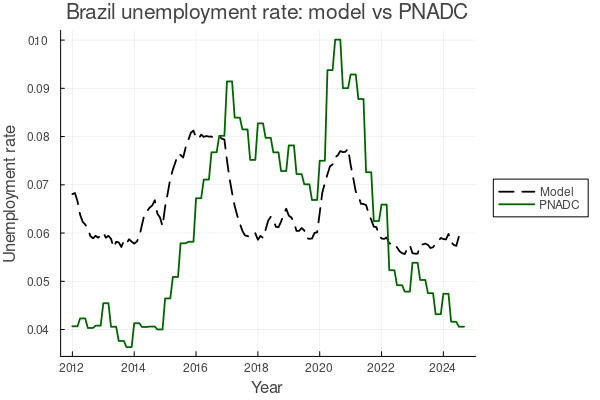
\includegraphics[width=0.48\linewidth]{model_vs_pnadc_unemployment.png}}
		\hfill
		\subfigure[Participation rate.\label{fig:model-vs-pnadc-participation}]{%
			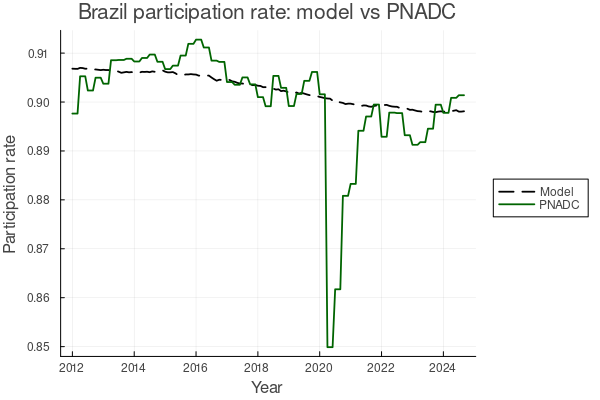
\includegraphics[width=0.48\linewidth]{model_vs_pnadc_participation.png}}
		\caption{Labor-market moments: model versus PNAD-C for the full trial-6 wage/skill candidate. Unemployment remains close on average, but participation falls below PNAD-C after changing the wage process.}
	\end{figure}

	Figures \ref{fig:model-vs-rais-percentiles} and \ref{fig:model-vs-rais-ratios} compare the RAIS formal earnings moments with the RAIS-comparable model object. This comparison is conceptually cleaner than the previous version because the model percentiles are no longer contaminated by nonemployment or the minimum-income floor. The trial-6 candidate improves the upper tail of the employed-wage distribution relative to the inherited HPV wage block, but it over-spreads the lower half of the distribution.

	\begin{figure}[H]
		\centering
		\subfigure[Employed-wage percentiles.\label{fig:model-vs-rais-percentiles}]{%
			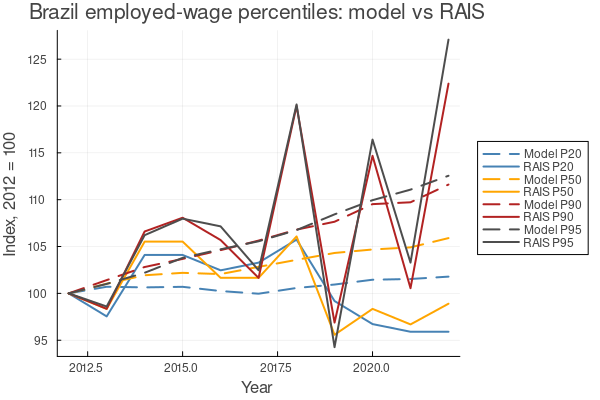
\includegraphics[width=0.48\linewidth]{model_vs_rais_percentiles.png}}
		\hfill
		\subfigure[Percentile ratios.\label{fig:model-vs-rais-ratios}]{%
			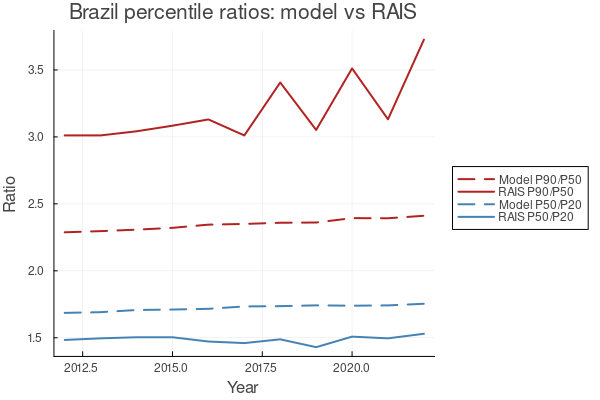
\includegraphics[width=0.48\linewidth]{model_vs_rais_percentile_ratios.png}}
		\caption{RAIS-comparable earnings moments: model versus RAIS. Percentiles are indexed to the first common year, and ratios are computed from employed-wage percentiles.}
	\end{figure}

	\begin{table}[H]
		\centering
		\caption{RAIS Wage Fit: Full Trial-6 Candidate}
		\label{tab:rais-wage-fit-trial6}
		\small
		\begin{tabular}{lccc}
			\toprule
			Moment & Model endpoint & RAIS endpoint & Fit statistic \\
			\midrule
			P20 index & 94.94 & 95.90 & 4.728 \\
			P50 index & 101.15 & 98.90 & 3.441 \\
			P90 index & 113.27 & 122.39 & 7.134 \\
			P95 index & 117.55 & 127.08 & 8.222 \\
			P90/P50 ratio & 3.119 & 3.726 & 0.282 \\
			P50/P20 ratio & 2.023 & 1.530 & 0.480 \\
			\bottomrule
		\end{tabular}
		\caption*{Notes: Percentile indexes are normalized to the first common year, 2012. Fit statistics are index RMSEs for percentile paths and level RMSEs for percentile ratios over 2012--2022.}
	\end{table}

	The main limitation of the current exercise is that the labor-market block and the wage distribution have not yet been estimated jointly. The trial-6 candidate shows that raising initial wage dispersion and the trend in dispersion can substantially improve the upper-tail ratio, especially P90/P50. At the same time, it raises P50/P20 too much and lowers participation below the PNAD-C target. The next iteration should therefore estimate participation and wage-process parameters jointly, with a loss function that targets PNAD-C unemployment and participation together with RAIS percentile paths and ratios.

	\section{Conclusion and Remaining Work} \label{sec:conclusion}

	The current Brazil version of the model delivers two useful intermediate conclusions. First, the PNAD-C labor-market block is internally consistent and quantitatively close to the Brazilian data for prime-age men when evaluated as the Brazil v2 labor baseline. This suggests that the basic Brazilian transition structure is viable. Second, the first RAIS wage/skill candidate improves the fit of the upper tail of the formal wage distribution, but it also worsens participation and the lower-half wage ratio. This shows that the labor and wage blocks cannot be finalized sequentially.

	A second conclusion is conceptual. RAIS and the all-population earnings object must remain separate throughout the analysis. RAIS measures earnings among formal jobs, while the HPV model also produces an annual earnings object that includes nonemployment and income floors. Comparing RAIS percentiles with an all-population object would mechanically confound wage inequality with employment and participation margins. The current implementation corrects this issue by constructing RAIS-comparable employed-wage moments inside the model.

	The current version should not yet be interpreted as a final quantitative result on the evolution of Brazilian earnings inequality. The trial-6 wage/skill candidate is informative because it moves the model in the right direction for P90/P50, but it does not provide an acceptable joint fit. The evidence so far is strongest for three points: the feasibility of the Brazilian transition block, the importance of separating formal-job earnings from all-population earnings, and the need for a joint calibration of participation and wage dispersion.

	Substantively, the model points to recessions affecting earnings through two channels. The first is the employment-margin channel: adverse aggregate states reduce the probability of moving into employment and, in crisis periods, raise the probability of job loss, especially for low-skill workers. This lowers current labor income and increases the time spent without earnings. The second is the dynamic skill channel: nonemployment depreciates skills through $\delta^-$, while employment increases future skills through $\delta^+$. Recessions therefore have persistent effects because a temporary job loss can lower future earning capacity, not only contemporaneous income.

	The participation margin works in the same direction. When job-finding probabilities fall and expected wages are lower, the value of searching falls relative to non-participation. The model therefore predicts that recessions can induce some workers, especially those with low skills or high taste for leisure, to leave the labor force. In the current trial-6 calibration this mechanism is too strong: aggregate participation falls below PNAD-C in every aggregate state. This overreaction is informative for calibration, because it shows that the wage process and participation block must be estimated jointly rather than sequentially.

	\begin{table}[H]
		\centering
		\caption{Remaining Work After the Current Brazil Candidate}
		\label{tab:remaining-work-current-candidate}
		\small
		\begin{tabular}{p{0.27\linewidth}p{0.31\linewidth}p{0.31\linewidth}}
			\toprule
			Task & Current status & Required next step \\
			\midrule
			Labor-market fit & The Brazil v2 labor baseline matches PNAD-C averages, but the trial-6 wage candidate lowers participation. & Re-estimate participation parameters jointly with the wage process. \\
			Worker types & PNAD-C transitions are loaded for low-, mid-, and high-skill workers. & Allow wage-process parameters or initial skill distributions to vary by education group. \\
			RAIS comparison & Trial 6 improves P90/P50 but overstates P50/P20 and still underpredicts P90 and P95 growth. & Run a finer local search that preserves the upper-tail gain while reducing the lower-half spread. \\
			Joint calibration & Labor moments and wage moments are still treated mostly sequentially. & Estimate a joint loss function targeting PNAD-C unemployment, PNAD-C participation, and RAIS earnings moments. \\
			Robustness & Aggregate states are based on the current cycle classification. & Compare results using alternative boom definitions, CODACE dating, and specifications excluding 2020. \\
			Reproducibility & The Brazil v2 labor baseline and the trial-6 RAIS wage candidate are saved as snapshots. & Freeze the next accepted candidate only after the joint calibration improves both participation and RAIS ratios. \\
			\bottomrule
		\end{tabular}
		\caption*{Notes: The current candidate refers to the full trial-6 wage/skill run documented in Section \ref{sec:preliminary-fit}. The next version should treat the labor and wage blocks as a single estimation problem.}
	\end{table}

	The next version of the paper should therefore move from a block-by-block calibration to a fully calibrated distributional exercise. Once participation and the wage process are disciplined jointly by PNAD-C and RAIS, the model can be used to ask whether Brazilian business-cycle dynamics amplify or dampen earnings inequality across the formal labor market, and whether these effects differ from the U.S. mechanisms emphasized by HPV.
	
	
	\newpage
	
	\singlespacing
	\setlength\bibsep{0pt}
	\bibliographystyle{plainnat}
	\bibliography{references}
	
	
	
	\clearpage
	
	\onehalfspacing
	
	%\section{Appendix}
	
	
	
	%\section*{Tables} \label{sec:tab}
	%\addcontentsline{toc}{section}{Tables}
	
	
	
	%\clearpage
	
	%\section*{Figures} \label{sec:fig}
	%\addcontentsline{toc}{section}{Figures}
	
	%\begin{figure}[hp]
	%  \centering
	%  \includegraphics[width=.6\textwidth]{../fig/placeholder.pdf}
	%  \caption{Placeholder}
	%  \label{fig:placeholder}
	%\end{figure}
	
	
	
	
	%\clearpage
	
	%\section*{Appendix A. Placeholder} \label{sec:appendixa}
	%\addcontentsline{toc}{section}{Appendix A}
	
	
	
\end{document}
